% use options
%  '[beamer]' for a digital projector
%  '[trans]' for an overhead projector
%  '[handout]' for 4-up printed notes
\documentclass[beamer, compress]{beamer}

% change talk_preamble if you want to modify the slide theme, colours, and settings for trans and handout modes.
\newcommand{\pathtotrunk}{../../}
\input{\pathtotrunk preamble.tex}
%!TEX root = ../blob1.tex

%%%%% excerpts from KW's include file of standard macros

\def\z{\mathbb{Z}}
\def\r{\mathbb{R}}
\def\c{\mathbb{C}}
\def\t{\mathbb{T}}

\def\du{\sqcup}
\def\bd{\partial}
\def\sub{\subset}
\def\subeq{\subseteq}
\def\sup{\supset}
%\def\setmin{\smallsetminus}
\def\setmin{\setminus}
\def\ep{\epsilon}
\def\sgl{_\mathrm{gl}}
\def\op{^\mathrm{op}}
\def\deq{\stackrel{\mathrm{def}}{=}}
\def\pd#1#2{\frac{\partial #1}{\partial #2}}
\def\lf{\overline{\cC}}
\def\ot{\otimes}

\def\nn#1{{{\it \small [#1]}}}
\long\def\noop#1{}

% equations
\newcommand{\eq}[1]{\begin{displaymath}#1\end{displaymath}}
\newcommand{\eqar}[1]{\begin{eqnarray*}#1\end{eqnarray*}}
\newcommand{\eqspl}[1]{\begin{displaymath}\begin{split}#1\end{split}\end{displaymath}}

% tricky way to iterate macros over a list
\def\semicolon{;}
\def\applytolist#1{
    \expandafter\def\csname multi#1\endcsname##1{
        \def\multiack{##1}\ifx\multiack\semicolon
            \def\next{\relax}
        \else
            \csname #1\endcsname{##1}
            \def\next{\csname multi#1\endcsname}
        \fi
        \next}
    \csname multi#1\endcsname}

% \def\cA{{\cal A}} for A..Z
\def\calc#1{\expandafter\def\csname c#1\endcsname{{\mathcal #1}}}
\applytolist{calc}QWERTYUIOPLKJHGFDSAZXCVBNM;

% \DeclareMathOperator{\pr}{pr} etc.
\def\declaremathop#1{\expandafter\DeclareMathOperator\csname #1\endcsname{#1}}
\applytolist{declaremathop}{pr}{im}{gl}{ev}{coinv}{tr}{rot}{Eq}{obj}{mor}{ob}{Rep}{Tet}{cat}{Maps}{Diff}{Homeo}{sign}{supp}{Nbd};



%%%%%% end excerpt



\usepackage{etex}
\usepackage{pgfpages}

\usepackage{color}

\usepackage{tikz}
\usetikzlibrary{shapes}
\usetikzlibrary{backgrounds}

% beamer mode
\mode<beamer>{
\useinnertheme[shadow=true]{rounded}
\useoutertheme{shadow}
\usecolortheme{orchid}
\usecolortheme{whale}
\setbeamerfont{block title}{size={}}

\setbeamertemplate{headline}
{%
}

\setbeamertemplate{footline}
{%
  \leavevmode%
  \hbox{\begin{beamercolorbox}[wd=.25\paperwidth,ht=2.5ex,dp=1.125ex,leftskip=.3cm,rightskip=.3cm]{author in head/foot}%
    \usebeamerfont{author in head/foot}\insertshortauthor
  \end{beamercolorbox}%
  \begin{beamercolorbox}[wd=.25\paperwidth,ht=2.5ex,dp=1.125ex,leftskip=.3cm,rightskip=.3cm]{title in head/foot}%
    \usebeamerfont{title in head/foot}\insertshorttitle
  \end{beamercolorbox}}%
    \begin{beamercolorbox}[wd=.5\paperwidth,ht=2.5ex,dp=1.125ex]{section in head/foot}%
    \insertsectionnavigationhorizontal{.5\paperwidth}{}{\hskip0pt plus1filll}%
  \end{beamercolorbox}%
  \vskip0pt%
}

}



% transparency mode
\mode<trans>{
 \usetheme{Warsaw}
}

% handout mode
\mode<handout>{
 \usetheme{default}
 \setbeamercolor{background canvas}{bg=black!5}
 \pgfpagesuselayout{4 on 1}[letterpaper,landscape,border shrink=2.5mm]
}

\newcommand{\return}[2]{\hyperlink{#1}{\beamerreturnbutton{#2}}}
\newcommand{\goto}[2]{\hyperlink{#1}{\beamergotobutton{#2}}}
\newcommand{\skipto}[2]{\hyperlink{#1}{\beamerskipbutton{#2}}}

\beamertemplatetransparentcovered 
\setbeamertemplate{navigation symbols}{}  % no navigation symbols, please
\mode<beamer>{\setbeamercolor{block title}{bg=green!40!black}}
\beamersetuncovermixins 
{\opaqueness<1->{60}} 
{} 


% This switches fonts to the Palatino family.
%  \renewcommand{\familydefault}{ppl}

\usepackage{array}


%\setbeameroption{previous slide on second screen=right}

\author[Scott Morrison]{Scott Morrison \\ \texttt{http://tqft.net/} \\ joint work with Kevin Walker}
\institute{UC Berkeley / Miller Institute for Basic Research}
\title{The blob complex}
\date{
Low-Dimensional Topology and Categorification, \\
Stony Brook University, June 21-25 2010 \\
\begin{description}
	\item[slides:]\url{http://tqft.net/talks}
	\item[paper:]\url{http://tqft.net/blobs}
%	\item[shameless plug:]\url{http://mathoverflow.net}
\end{description}
}

\listfiles

\begin{document}

\frame{\titlepage}


\section{Overview}

   \begin{frame}<beamer>
       \frametitle{The blob complex}
       \begin{quote}
      ... homotopical topology and TQFT have grown so close that I have started thinking that they are turning into the language of new foundations. 
        \end{quote}
        \flushright{--- \href{http://www.ams.org/notices/200910/rtx091001268p.pdf}{Yuri Manin, September 2008}}
      \tableofcontents
\end{frame}

\begin{frame}{What is \emph{the blob complex}?}
\begin{block}{}
The blob complex takes an $n$-manifold $\cM$ and an `$n$-category with strong duality' $\cC$ and produces a chain complex, $\bc_*(\cM; \cC)$.
\end{block}
\tikzstyle{description}=[gray, font=\tiny, text centered, text width=2cm]
\begin{tikzpicture}[]
\setbeamercovered{%
 transparent=5,
% still covered={\opaqueness<1>{15}\opaqueness<2>{10}\opaqueness<3>{5}\opaqueness<4->{2}},
 again covered={\opaqueness<1->{50}}
}

\node[red] (blobs) at (0,0) {$H(\bc_*(\cM; \cC))$};
\uncover<2>{
\node[blue] (skein) at (4,0) {$\cA(\cM; \cC)$};
\node[below=5pt, description] (skein-label) at (skein) {(the usual TQFT Hilbert space)};
\path[->](blobs) edge node[above] {$*= 0$} (skein);
}

\uncover<3>{
  \node[blue] (hoch) at (0,3) {$HH_*(\cC)$};
  \node[right=20pt, description] (hoch-label) at (hoch) {(the Hochschild homology)};
  \path[->](blobs) edge node[right] {$\cM = S^1$} (hoch);
}

\uncover<4>{
  \node[blue] (comm) at (-2.4, -1.8) {$H_*(\Delta^\infty(\cM), k)$};
  \node[description, below=5pt] (comm-label) at (comm) {(singular homology of the infinite configuration space)};
  \path[->](blobs) edge node[right=5pt] {$\cC = k[t]$} (comm);
}

\end{tikzpicture}
\end{frame}

\section{TQFTs}

\begin{frame}{$n$-categories}
\begin{block}{There are many definitions of $n$-categories!}
For most of what follows, I'll draw $2$-dimensional pictures and rely on your intuition for pivotal $2$-categories. 
\end{block}
\begin{block}{We have another definition: \emph{topological $n$-categories}}
\begin{itemize}
%\item A set $\cC(B^k)$ for every $k$-ball, $0 \leq k < n$.
\item A vector space $\cC(B^n)$ for every $n$-ball $B$.
%\item From these, inductively
%\begin{itemize}
%\item define a set $\cC(S^k)$ for each $k$-sphere, $0 \leq k < n$,
%\item require a map $\cC(B^k) \to \cC(S^{k-1})$.
%\end{itemize}
\item An associative gluing map: with $B = \bigcup_i B_i$, balls glued together to form a ball,
$$\bigotimes \cC(B_i) \to \cC(B)$$
(the $\tensor$ is fibered over `boundary restriction' maps).
\item ...
\end{itemize}
\end{block}
These are easy to check for geometric examples, hard to check for algebraic examples.
\end{frame}

\begin{frame}{Cellulations of manifolds}
\begin{block}{}
Consider $\cell(M)$, the category of cellulations of a manifold $M$, with morphisms `antirefinements'.
\end{block}
\vspace{-4mm}
$$\mathfig{.35}{ncat/zz2}$$
\vspace{-4mm}
\begin{block}{}
An $n$-category $\cC$ gives a functor from $\cell(M)$ to vector spaces.
\begin{description}
\item[objects] send a cellulation to the product of $\cC$ on each top-cell, restricting to the subset where boundaries agree
\item[morphisms] send an antirefinement to the appropriate gluing map.
\end{description}
\end{block}
\end{frame}

\newcommand{\roundframe}[1]{\begin{tikzpicture}[baseline=-2pt]\node[rectangle,inner sep=1pt,rounded corners,fill=white] {#1};\end{tikzpicture}}

\begin{frame}{Fields}
\begin{block}{}
A field on $\cM^n$ is a choice of cellulation and a choice of $n$-morphism for each top-cell (with matching boundaries).
%$$\cF(\cM) = \bigoplus_{\cX \in \cell(M)} \bigotimes_{B \in \cX} \cC(B)$$
\end{block}
\begin{example}[$\cC = \text{TL}_d$ the Temperley-Lieb category]
$$\roundframe{\mathfig{0.35}{definition/example-pasting-diagram}} \in \cF\left(T^2\right)$$
\end{example}
\begin{block}{}
Given a field on a ball, we can evaluate it to a morphism using the gluing map. We call the kernel the \emph{null fields}.
\vspace{-3mm}
$$\text{ev}\Bigg(\roundframe{\mathfig{0.12}{definition/evaluation1}} - \frac{1}{d}\roundframe{\mathfig{0.12}{definition/evaluation2}}\Bigg) = 0$$
\end{block}
\end{frame}

\begin{frame}{Background: TQFT invariants}
\begin{defn}
We associate to an $n$-manifold $\cM$ the skein module
\vspace{-1mm}
$$\cA(\cM) = \cF(\cM) / \ker{ev},\vspace{-1mm}$$
fields modulo fields which evaluate to zero inside some ball.
\end{defn}
Equivalently, $\cA(\cM)$ is the colimit of $\cC$ along $\cell(M)$.

\vspace{4mm}
%\begin{itemize}
%\item We can also associate a $k$-category to an $n-k$-manifold.
%\item We don't assign a number to an $n+1$-manifold (a `decapitated' extended TQFT).
%\end{itemize}
$\cA(Y \times [0,1])$ is a $1$-category, and when $Y \subset \bdy X$, $\cA(X)$ is a module over $\cA(Y \times [0,1])$.
\begin{thm}[Gluing formula]
When $Y \sqcup Y^{\text{op}} \subset \bdy X$,
\vspace{-1mm}
\[
	\cA(X \bigcup_Y \selfarrow) \iso \cA(X) \bigotimes_{\cA(Y \times [0,1])} \selfarrow.
\]
\end{thm}
\end{frame}

\begin{frame}{Motivation: Khovanov homology as a $4$d TQFT}
\begin{thm}
Khovanov homology gives a $4$-category:
\begin{description}
\item[3-morphisms] tangles, with the usual $3$ operations,
\item[4-morphisms] $\Hom{Kh}{T_1}{T_2} = Kh(T_1 \cup \bar{T_2})$, composition defined by saddle cobordisms
\end{description}
\end{thm}
\begin{block}{}
There is a corresponding $4$-manifold invariant. Given $L \subset \bdy W^4$, it associates a doubly-graded vector space $\cA(W, L; Kh)$.
$$\cA(B^4, L; Kh) \iso Kh(L)$$
\end{block}
\end{frame}

\begin{frame}{Computations are hard}
\begin{block}{}
This invariant is hard to compute, because the TQFT skein module construction breaks the exact triangle for resolving a crossing.
\vspace{-0.3cm}
\begin{align*}
\begin{tikzpicture}
\node(a) at (0,0) {$Kh\left(\begin{tikzpicture}[baseline=-2.5pt, scale=0.5, line width=1.5pt]
\node[outer sep=-1pt] (x) at (0,0){};
    \draw (x.45)-- (.5,.5);
    \draw (x.135) -- (-.5,.5);
    \draw (x.315) -- (.5,-.5);
    \draw (x.45) -- (-.5,-.5);
\end{tikzpicture}\right)$};
\node(b) at (-1.2,-1.5) {$Kh\left(
\begin{tikzpicture}[baseline=-2.5pt, scale=0.5, line width=1.5pt]
    \draw (1.5,.5) .. controls (2,0) .. (1.5,-.5);
    \draw (2.5,.5) .. controls (2,0) .. (2.5,-.5);
\end{tikzpicture}\right)$};
\node(c) at (1.2,-1.5) {$Kh\left(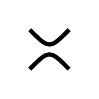
\begin{tikzpicture}[baseline=-2.5pt, scale=0.5, line width=1.5pt]
    \draw (3.5,.5) .. controls (4,0) .. (4.5,.5);
    \draw (3.5,-.5) .. controls (4,0) .. (4.5,-.5);
\end{tikzpicture}\right)$};
\draw[->] (a) -- (b);
\draw[->] (b) -- (c);
\draw[->] (c) -- (a);
\end{tikzpicture}
\qquad \qquad
\begin{tikzpicture}
\node(a) at (0,0) {$\cA\left(M, \begin{tikzpicture}[baseline=-2.5pt, scale=0.5, line width=1.5pt]
\node[outer sep=-1pt] (x) at (0,0){};
    \draw (x.45)-- (.5,.5);
    \draw (x.135) -- (-.5,.5);
    \draw (x.315) -- (.5,-.5);
    \draw (x.45) -- (-.5,-.5);
\end{tikzpicture}\right)$};
\node(b) at (-1.4,-1.5) {$\cA\left(M, 
\begin{tikzpicture}[baseline=-2.5pt, scale=0.5, line width=1.5pt]
    \draw (1.5,.5) .. controls (2,0) .. (1.5,-.5);
    \draw (2.5,.5) .. controls (2,0) .. (2.5,-.5);
\end{tikzpicture}\right)$};
\node(c) at (1.4,-1.5) {$\cA\left(M,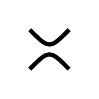
\begin{tikzpicture}[baseline=-2.5pt, scale=0.5, line width=1.5pt]
    \draw (3.5,.5) .. controls (4,0) .. (4.5,.5);
    \draw (3.5,-.5) .. controls (4,0) .. (4.5,-.5);
\end{tikzpicture}\right)$};
\node at (0,-0.75) {\Large \color{red} ?};
\draw[dashed] (a) -- (b);
\draw[dashed] (b) -- (c);
\draw[dashed] (c) -- (a);
\end{tikzpicture}
\end{align*}\vspace{-1cm}
\end{block}
There is a spectral sequence converging to $0$ relating the blob homologies for the triangle of resolutions. 
\begin{conj}
It may be possible to compute the skein module
%$$\cA(W, L; Kh) = H_0(\bc_*(W, L; Kh))$$
by first computing the entire blob homology.
\end{conj}
\end{frame}

\section{Definition}
\begin{frame}{\emph{Definition} of the blob complex, $k=0,1$}
\begin{block}{Motivation}
A \emph{local} construction, such that when $\cM$ is a ball, $\bc_*(\cM; \cC)$ is a resolution of $\cA(\cM; \cC)$.
\end{block}

\mode<handout>{\vspace{-5mm}}
\begin{block}{}
\center
$\bc_0(\cM; \cC) = \cF(\cM)$, arbitrary fields on $\cM$.
\end{block}

\begin{block}{}
\vspace{-1mm}
$$\bc_1(\cM; \cC) = \Complex\setcr{(B, u, r)}{\begin{array}{c}\text{$B$ an embedded ball}\\\text{$u \in \cF(B)$ in the kernel}\\ r \in \cF(\cM \setminus B)\end{array}}.$$
\end{block}
\vspace{-3.5mm}
$$\mathfig{.5}{definition/single-blob}$$
\vspace{-3mm}
\begin{block}{}
\mode<handout>{\vspace{-5mm}}
\vspace{-6mm}
\begin{align*}
d_1 : (B, u, r) & \mapsto u \circ r & \bc_0 / \im(d_1) \iso A(\cM; \cC)
\end{align*}
\end{block}
\end{frame}

\begin{frame}{Definition, $k=2$}
\begin{block}{}
\vspace{-1mm}
\mode<handout>{\vspace{-5mm}}
$$\bc_2 = \bc_2^{\text{disjoint}} \oplus \bc_2^{\text{nested}}$$
\end{block}
\begin{block}{}
\mode<handout>{\vspace{-5mm}}
\vspace{-5mm}
\begin{align*}
\bc_2^{\text{disjoint}} & =  \Complex\setcl{\roundframe{\mathfig{0.5}{definition/disjoint-blobs}}}{\text{ev}_{B_i}(u_i) = 0}
\end{align*}
\vspace{-4mm}
$$d_2 : (B_1, B_2, u_1, u_2, r) \mapsto (B_2, u_2, r \circ u_1) - (B_1, u_1, r \circ u_2)$$
\end{block}
\begin{block}{}
\vspace{-5mm}
\begin{align*}
\bc_2^{\text{nested}} & = \Complex\setcl{\roundframe{\mathfig{0.5}{definition/nested-blobs}}}{\text{ev}_{B_1}(u)=0}
\end{align*}
\vspace{-4mm}
$$d_2 : (B_1, B_2, u, r', r) \mapsto (B_2, u \circ r', r) - (B_1, u, r \circ r')$$
\end{block}
\end{frame}

\begin{frame}{Definition, general case}
\begin{block}{}
$$\bc_k = \Complex\set{\roundframe{\mathfig{0.7}{definition/k-blobs}}}$$
$k$ blobs, properly nested or disjoint, with ``innermost'' blobs labelled by fields that evaluate to zero.
\end{block}
\begin{block}{}
\vspace{-2mm}
$$d_k : \bc_k \to \bc_{k-1} = {\textstyle \sum_i} (-1)^i (\text{erase blob $i$})$$
\end{block}
\end{frame}

\section{Properties}
\begin{frame}{Hochschild homology}
\begin{block}{TQFT on $S^1$ is `coinvariants'}
\vspace{-3mm}
$$\cA(S^1, A) = \Complex\set{\roundframe{
\tikz{\draw (0,0) circle (0.4); \foreach \q/\l in {90/a, 210/b, 330/c} {\draw[fill=red] (\q:0.4) circle (0.075); \node at (\q:0.6) {\l};}}
}}
\scalebox{2}{$/$}
\set{\roundframe{\tikz{\draw (-30:0.4) arc (-30:210:0.4); \draw[fill=red] (90:0.4) circle (0.075); \node at (90:0.65) {$ab$};}} - \roundframe{
\tikz{\draw (-30:0.4) arc (-30:210:0.4); \foreach \q/\l in {120/a, 60/b} {\draw[fill=red] (\q:0.4) circle (0.075); \node at (\q:0.65) {\l};}}}} = A/(ab-ba)$$
\end{block}
\mode<handout>{\vspace{-3mm}}
\begin{block}{Blob homology on $S^1$ is Hochschild homology}
The Hochschild complex is `coinvariants of the bar resolution'
\vspace{-2mm}
$$ \cdots \to A \tensor A \tensor A \to A \tensor A \xrightarrow{m \tensor a \mapsto ma-am} A$$

We check universal properties, as it's hard to directly construct an isomorphism.
\noop{
$$m \tensor a \mapsto
\roundframe{\mathfig{0.35}{hochschild/1-chains}}
$$
\vspace{-5mm}
\begin{align*}
u_1 & = \mathfig{0.05}{hochschild/u_1-1} - \mathfig{0.05}{hochschild/u_1-2} & u_2  &= \mathfig{0.05}{hochschild/u_2-1} - \mathfig{0.05}{hochschild/u_2-2} 
\end{align*}
}
\end{block}
\end{frame}

\begin{frame}{An action of $\CH{\cM}$}
\begin{thm}
There's a chain map
$$\CH{\cM} \tensor \bc_*(\cM) \to \bc_*(\cM).$$
which is associative up to homotopy, and compatible with gluing.
\end{thm}
\begin{block}{}
Taking $H_0$, this is the mapping class group acting on a TQFT skein module.
$$H_0(\Homeo(\cM)) \tensor \cA(\cM) \to \cA(\cM).$$
\end{block}
\end{frame}

\mode<beamer>{
\begin{frame}{An action of $\CH{\cM}$}
\begin{proof}
\begin{description}
\item[Step 1] If $\cM=B^n$ or a union of balls, there's a unique chain map, since $\bc_*(B^n; \cC) \htpy \cC$ is concentrated in homological degree $0$.
\item[Step 2] Fix an open cover $\cU$ of balls. \\ A family of homeomorphisms $P^k \to \Homeo(\cM)$ can be broken up in into pieces, each of which is supported in at most $k$ open sets from $\cU$. \qedhere
\end{description}
\end{proof}
\end{frame}
}

\begin{frame}{Gluing}
\begin{block}{$\bc_*(Y \times [0,1])$ is naturally an $A_\infty$ category}
\begin{description}
\item[multiplication ($m_2$):] gluing $[0,1] \simeq [0,1] \cup [0,1]$
\item[associativity up to homotopy ($m_k$):] reparametrising $[0,1]$ using the action of $\CH{[0,1]}$.
\end{description}
\end{block}
\begin{block}{}
If $Y \subset \bdy X$ then $\bc_*(X)$ is an $A_\infty$ module over $\bc_*(Y)$.
\end{block}
\begin{thm}[Gluing formula]
When $Y \sqcup Y^{\text{op}} \subset \bdy X$,
\vspace{-5mm}
\[
	\bc_*(X \bigcup_Y \selfarrow) \iso \bc_*(X) \bigotimes_{\bc_*(Y)}^{A_\infty} \selfarrow.
\]
\end{thm}
In principle, we can compute blob homology from a handle decomposition, by iterated Hochschild homology.
\end{frame}

\begin{frame}{Higher Deligne conjecture}
\begin{block}{Deligne conjecture}
Chains on the little discs operad acts on Hochschild cohomology.
\end{block}

\begin{block}{}
Call $\Hom{\bc_*(\bdy M)}{\bc_*(\cM)}{\bc_*(\cM)}$ `blob cochains on $\cM$'.
\end{block}

\begin{block}{Theorem (Higher Deligne conjecture)}
\scalebox{0.96}{Chains on the $n$-dimensional fat graph operad acts on blob cochains.}
\vspace{-3mm}
$$\mathfig{.85}{deligne/manifolds}$$
\end{block}
\end{frame}

\begin{frame}{Maps to a space}
\begin{block}{}
Fix a target space $\cT$. There is an $A_\infty$ $n$-category $\pi_{\leq n}^\infty(\cT)$ defined by
$$\pi_{\leq n}^\infty(\cT)(B) = C_*(\Maps(B\to \cT)).$$
(Here $B$ is an $n$-ball.)
\end{block}
\begin{thm}
The blob complex recovers mapping spaces:
$$\bc_*(\cM; \pi_{\leq n}^\infty(\cT)) \iso C_*(\Maps(\cM \to \cT))$$
\end{thm}
This generalizes  a result of Lurie: if $\cT$ is $n-1$ connected, $\pi_{\leq n}^\infty(\cT)$ is an $E_n$-algebra and in this special case the blob complex is presumably the same as his topological chiral homology.
\end{frame}

\end{document}
% ----------------------------------------------------------------

